\chapter{Mildstone implementation details}
\label{section:5_mildstone}
% \section{Mildstone \\ \small{ a framework for learning within the machine }}
% explain why it is needed ( of worth ) the complete redesign for a new acquisition chain.
% explain why we need a framework for that.
% tensorflow
% MDSplus, MARTe
% ...

During the study of ML algorithms for this research, a complex set of tools have been used revealing a difficult organization of the needed components.
This is indeed one of the main difficulties that characterize the ML study nowadays, and one of the reasons that discourage its use on the context of physics and control.
One of the key aspects to apply this paradigm is thus to organize the use of algorithms in a way that all changes must be tracked and all tests can be compared.
Moreover the statistical intimate basis of them forces the organization of the data as well, to provide a fast and accurate access to experiment measures. 
Last but not least, the heterogeneity of the host architecture where the network can be trained, tested, and deployed asks for a extreme flexibility of the algorithms implementation.

These three factors suggested that, for the real application of such tools in the context of an experimental facility, a unique organization of the overall structure of the code repository, data storing, and architecture deployment become necessary.
In fusion community some big infrastructure have been already adopted for data acquisition and control systems (CODAS), for instance the ITER CODAC tools~\cite{iter_CODAC} represents the current main attempt to a complete unification and integration of the software components needed at ITER.
On the other hand the dynamicity of ML evolution requires to have a smaller and yet flexible environment that can be easily made compatible with the rapid changes that the community of developers propose.
A interesting meter of the evolution rate in the context of ML is the publication target of such works, that in the almost totality of the cases is addressed to the public access repositories without even being peer reviewed, or at least the with open-reviewing systems~\cite{open_review}. 


% schema a blocchi con:
% DAQ -> Digital Post-conditionining - Data Storage -> Data integration device -> Model integration device -> Controller
% Code Storage .. and Code auditing tools (the chance to acquire status for all components)
%

\section{Tensorflow}

\Tensorflow framework~\cite{tensorflow2015-whitepaper} has been designed as an interface for machine learning algorithms containing the implementations for many of them and a base of execution. A computation can be executed in \Tensorflow with little or no changes on a wide variety of hardware architectures and operative systems, ranging from embedded devices up to large-scale distributed systems for parallel computation. The system is flexible enough to express a wide variety of models: this includes training and inference algorithms for \acs{DNN}, and it can be used for conducting research and for deploying in production environment. 
The beauty of the framework definition is that it has been meant to provide an abstract definition of the algorithms by means of representative interfaces. Once these interface have been implemented and instantiated, it also provides a way of handling the message passing among instances composing and handling complex "flow" of data. In this way a single script, for example written in python, can handle a wide set of distributed computation, where the specific implementation appears almost hidden to the user but is able to adapt to extreme hardware optimization underneath.

The idea of a single definition for transferring data among distributed system is not a real novelty though. This is actually the key component for a distributed system and many attempt have been made to create a unique representation for that. 
%Some publicly available like OpenORB D-BUS ~\cite{} some not DCE, COM, ZeroC
This holds also for tools that are already been adopted by fusion community. For example the MDSplus data acquisition system uses a unified definition of exchanged types as well, called "descriptors", that is in turn inspired by the internal structures of the Digital-VMS system.

%The idea of embracing \Tensorflow comes on one side from the widespread utilization on the ML community




\section{Anacleto - embedded FPGA development}

The use of FPGA-based solutions in data acquisition and control systems (CODAS) for nuclear fusion devices has been rather limited in the past compared to other physics experiments such as accelerators. This fact is mainly due to the different requirements: while in accelerators it is necessary to manage a large number of fast events from the detectors, which require a rapid reduction of data on the fly based on coincidences, in the fusion experiments a smaller number of channels is used, and generally requires the acquisition of input signals for data storage and possibly real-time control. 
Therefore, the fusion experiment uses more conventional electronic devices such as transient recorders, replaced in recent long-term experiments from analog to digital devices (ADCs) that support a continuous output data stream. Furthermore, the dynamics of the phenomena controlled in real time, such as the stability of the plasma, in most cases requires a response time of the order of milliseconds, while the control of the fastest phenomena such as vertical stabilization in tokamak requires a time of response of the order of 100$\mu s$. These requirements can be met using current information technology, thus making the use of computers for general purposes preferable to specialized FPGA solutions. The development of FPGA solutions requires expertise and experience in hardware interfaces and hardware description (HDL). Considering also that the integration of custom FPGA systems in CODAS normally requires the development of some kind of specialized communication protocol, the amount of human resources needed to implement such solutions is often inaccessible, especially in small laboratories. For this reason, in the past FPGA solutions have been limited to specific applications in diagnostics~\cite{ana_1,ana_2}. A notable exception is certainly represented by the FPGA RIO architectures~\cite{ana_3} (Compact RIO and Flex RIO) which provide easy programming and FPGA integration through LabVIEW and have been widely adopted for plasma control~\cite{ana_4} and other diagnostic applications~\cite{ana_5} . This solution, proposed by National Instruments, aims to exploit the power of FPGA by removing the main barriers in their use, or the experience required in HDL programming and interfacing with the rest of the system. However, this solution is rather expensive and closed to the specific choice in the hardware and programming environment. A new modern approach to the integration of high-level software components with the power of logical FPGA design is gaining increasing attention in the integrated technologies market and exploits the System on Chip (SoC) solution that combines different hardware devices on the same chip. The main hardware competitors driving the FPGA SoC market are Intel / Altera and Xilinx, both offering almost the same development solutions but with their own proprietary software. In particular, the XILINX Zynq architecture~\cite{ana_6}, which implements an ARM processor and a configurable FPGA in the same chip, is a valuable candidate technology for a variety of applications of interest in fusion research, in which the fast FPGA logic can be combined with the software functions performed by a CPU for high level functions and communications.

A considerable number of heterogeneous hardware from many vendors has been released to the advantage of the high integration of SoC devices. The main advantages that these chips offer to programmable logic are the ability to interface and share hardware features typical of a complete system such as the DMA controller and external interfaces such as Ethernet or SATA.

Many software solutions have also been proposed, to guide the developer through the non-trivial mechanisms of the FPGA at the system interface, in addition to covering different programming approaches: from the low-level synthesis of the Verilog and VHDL hardware description, to the toolchains higher level than compiling real programming languages like SystemC OpenCL and others~\cite{ana_7,ana_8}.

For enable Mildstone to integrate with such heterogeneous solutions we designed yet another choice called Anacleto (Another automatic configuration for logical evaluation toolchain)~\cite{RIGONI2018122}. It is meant to be particularly targeted to the embedded GNU Linux devices, it was developed by the RFX consortium within this research study, and aims to propose a standard unified work-flow to the FPGA developer for programming both logic and software components in a uniform and portable way.

It is worth noting that in the development of the SoC Anacleto projects the knowledge of HDL, unlike other solutions such as the LabView interface of National Instrument RIO, is not hidden by the framework. The purpose of this framework is not to provide a new programming interface, adding another level of logic representation, but to facilitate the development process with well-known open source build tools. In this way Anacleto can be though as a way to access, easily and uniformly, to the low-level FPGA programming devices, and a much cheaper solution than RIO. Furthermore, at this level of low-abstraction, many of the features that are commonly used are already provided for free by chip suppliers, or with a reasonable license fee from external contributions, keeping a door open to a broad market of existing solutions.

The first candidate applications for SoC devices are timing systems, data acquisition preprocessing and fast calculation. Timing systems represent a classic field of FPGA applications and have been implemented both in customized systems~\cite{ana_9} and in commercial products~\cite{ana_10}. A typical timing application uses a synchronized synchronization signal distributed, normally via optical fiber, to all timing devices and possibly propagating asynchronous events. The FPGA provides the generation of the required timing signals (clock, trigger, ...) based on the current configuration loaded into the system using a sort of hardware interface such as PCI. In this case, a processor would introduce greater flexibility in managing the configuration, allowing, for example, to load the configuration via the network.

The integration of configurable FPGAs in data acquisition would provide much more flexibility in data management by introducing features not currently supported by ADC devices. An example is the possibility to manage the deferred triggers communicated via the network. The use of the network to communicate triggers in data acquisition introduces delays that can compromise the accuracy in the reconstruction of the acquired signal. However, if a trigger message also carries the exact trigger time and assuming that all devices have a precise knowledge of the time (for example using the IEEE 1588 timing protocol), it is possible to provide a correct reconstruction of the signal using a circular buffer internal maintaining a signal history that lasts at least the delay in trigger communication~\cite{ana_11}. The use of a configurable FPGA in data acquisition could also allow a significant reduction of the required front-end when integrated signals from electromagnetic probes are acquired. In this case it would be possible to avoid analogue integration before data acquisition by moving the integration into FPGA processing during acquisition.

The rapid calculation performed by FPGA allows more sophisticated algorithms to be used in real-time plasma control while maintaining the flexibility provided by a computer system. The same approach could be used for new data processing algorithms such as detection of functionality from acquired video frames. In this case the processor would supervise the data transfer and the FPGA would perform an intensive calculation for the detection of the functionalities. It is worth emphasizing that FPGA solutions are more difficult to develop than CPU-based solutions.

\subsubsection*{Software organization}
Anacleto uses the Autotools build infrastructure~\cite{ana_13} to organize the more general FPGA workflow that acts as a collection of standard GNU-driven toolchains. The development process remains rather complex because many components in the final device card must be orchestrated (i.e. kernel configuration, driver customization to manage the newly created device and so on) but the compilation is managed almost automatically and, once the project is correctly defined, all the steps are covered by the Makefile destinations that can be concatenated in a single execution. To develop a SoC application, you must first select the hardware system. Since we decided to use the Xilinx Zynq devices, as a first attempt, three low-cost solutions were considered: RedPitaya~\cite{ana_14}, ZedBoard~\cite{ana_15} and Parallella~\cite{ana_16}. RedPitaya is designed to be used as an autonomous system for the management of digital and analogue I / O signals. This card hosts ready-to-use ADC and DAC components and therefore may be more suitable for the development of small stand-alone applications, but for the same reason it shows reduced flexibility compared to the other two for the configuration of the I / O pins. The other cards are destined to be housed in a carrier board and therefore do not have additional I / O devices. In particular, Parallella addresses the calculation of high intensity applications and hosts an additional processor with 16 cores.

Several other software components, all free, are necessary for the development of a SoC application and its distribution on the target board. First of all, the VIVADO IDE (Integrated Development Environment) tool for HDL programming must be downloaded from XILINX (Verilog and VHDL are the supported languages). To be used on a specific target, VIVADO requires a specific target configuration, provided by the developer of the board, which specifies how the processor is configured in that particular board. Currently only the Red Pitaya configuration in the framework is managed, but it is expected that the Zed Board and Parallella configuration files will be included, adding the choice of the target board in the configuration phases. VIVADO provides a set of configurable intellectual property (IP) components that perform connectivity between the processor (ARM Cortex A9 dual core in the Zynq chip mounted on Red Pitaya) and the FPGA application. When no DMA is involved, communication between the processor and the FPGA application is performed by a configurable number of 32-bit registers and, optionally, one or more interrupt lines. When the developer creates a new project for an FPGA application, the IDE creates a set of IP components, performing handshaking with the internal bus (AXI bus) used to exchange information between the processor and the FPGA application. The IDE provides the definition of a set of 32-bit signals that can be used by the FPGA application for communication. In a typical use case, these signals will represent the configuration to be loaded in the FPGA application, but can also be used to exchange input and output data. After developing the specific application, the IDE will generate the binary code to be downloaded into the FPGA. Other configurable IP components provided by VIVADO allow the definition of up to two DMA channels for FPGA applications that manage data streaming.

The interface configuration, ie the number of shared registers, break lines and DMA channels must also be reflected in the memory map of the processor device. XILINX provides a github project that hosts an adapted version of the Linux 4.4 kernel in a Debian distribution. The project includes the toolchain for the ARM processor and the kernel sources and a tool for generating the device tree structure, used by Linux Kernel 4.4 for device abstraction~\cite{ana_17}. Basically, a description of the device tree provides information about connected devices, including memory addresses and device register sizes. In this case, the description of the device tree will include the registers used to communicate with the FPGA application. The device-specific tree for the Zynq chip is generated by the current VIVADO project from the Hardware Software Interface component belonging to the XILINX system development kit. The same component can generate models for the implementation of Bare Metal, Linux and FreeRTOS. In particular, the Linux driver model is generated in the framework based on the type of data transfer selected (mapped registers and / or DMA).

Once Linux is created and the corresponding device tree, the final step is the development, starting from the generated model, of a Linux device driver that will allow user programs to interact with the FPGA application. In the simplest configuration, a buffer in user space is mapped to the sets of registers defined in the FPGA application so that information is exchanged by reading and writing that buffer.

From the description above, it is clear that building a SoC system from scratch is not an easy task, despite the availability in the network of all the required tools. The presented framework integrates all the previous steps and greatly simplifies the overall process. In particular, the framework:
\begin{itemize}
    \item Supervises the compilation of the toolchain and the Linux kernel using the components taken from the XILINX repository;
    \item Manages the management of the VIVADO project and the IP components required for FPGA integration;
    \item It supervises the construction of the device tree necessary for the correct mapping of the FPGA registers in the address space of the processor;
    \item Provides models for the development of the required Linux drivers.
\end{itemize}


\begin{figure}
    \centering
    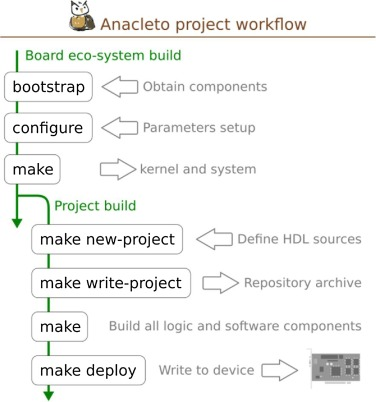
\includegraphics[height=5cm]{img/anacleto.jpg}
    \caption{Anacleto steps in building a new system. }
    \label{fig:anacleto_steps}
\end{figure}
Using this framework, a SoC FPGA application can be built from scratch by executing the general steps described in \Figure{\ref{fig:anacleto_steps}}:
As shown in the schema, the overall workflow can be splitted in two main stages: the building of the board system comprising the operating system kernel and software, and the specific project building with the definition of the logic and the software drivers that compile against the built kernel. The same board system can be shared among different specific projects and many different projects can be also installed in the same board. The reported steps depict a possible procedure example through the development process a developer would follow, that is:

\begin{itemize}
    \item \textbf{boostrap} the repository that set-up the environment and download all the required components and tools;
    then \textbf{configure} to set-up the system before building the toolchain and the Linux Kernel; this also compiles and shows a graphical user interface that eases the selection of the required options.

    \item \textbf{make} to compile the toolchain and then the Linux Kernel;
    
    \item \textbf{make new-project} to start a new VIVADO project for the development of the specific FPGA components in VHDL or Verilog. All the IP components required for SoC interface are created and can now be configured using VIVADO graphical        interface;
    
    \item \textbf{make write-project} once the logic has been defined with external sources and VIVADO project block designs, the whole project definition can be stored in the repository in the form of a script able to regenerate the project from scratch, even using different versions of VIVADO.
    
    \item At this point the FPGA application can be developed. It is also necessary to write the Linux driver for communication and a skeleton Linux driver source file is generated by the framework, based on the current configuration of the interface IP components. Then make starts both the logic synthesis and the compilation of software components.
    
    \item \textbf{make deploy} to generate the device-tree, compile the Kernel module, download the kernel and the bitstream into the target device.
    
\end{itemize}

The applicability of the SoC architecture has been further improved by the presented framework, hiding to the developer several intermediate steps and exposing only the necessary information for the proper system configuration. The presented framework however leaves to the developer the whole responsibility of the FPGA firmware development, a task that requires ingenuity and experience. 
There are however several applications of interest in fusion that don’t require sophisticated FPGA firmware, as it has been the case of the presented timing board. This class of applications is likely to benefit from SoC architecture, especially when the set of required tools and configurations is transparently managed by a tool like the one presented here.




% \section{Kinds of communication channel}
% \section{Mim - Mildstone approach for interface modelling}
